\documentclass[a4paper]{article}

\renewcommand{\labelenumii}{\theenumii}
\renewcommand{\theenumii}{\theenumi.\arabic{enumii}.}

\usepackage{fullpage} % Package to use full page
\usepackage{parskip} % Package to tweak paragraph skipping
\usepackage{tikz} % Package for drawing
\usepackage{amsmath}
\usepackage{amssymb,amsthm}
\usepackage{mathtools}
\usepackage{hyperref}
\usepackage{enumitem}
\usepackage{mathtools}
\usepackage{empheq}
\usepackage{amsfonts}
\usepackage{gensymb}
\usepackage{float}
\usepackage{subcaption}
\usepackage{placeins}
\usepackage{graphicx}


\newcommand*\widefbox[1]{\fbox{\hspace{2em}#1\hspace{2em}}}
%======================================== Title===========================================
\newcommand{\horrule}[1]{\rule{\linewidth}{#1}} 	% Horizontal rule
\title{
		\vspace{-0.6in} 	
		\usefont{OT1}{bch}{b}{n}
		\normalfont \normalsize \textsc{University of California Santa Cruz} \\ [10pt]
		\horrule{0.5pt} \\[0.4cm]
		\huge CMPE264 Project 2: Sweeping Plane Stereo \\
		\horrule{2pt} \\[0.5cm]
}
\author{
		\normalfont 								
        Aaron Hunter\\  Carlos Espinosa\\[-3pt]		\normalsize
}
%====================================Begin document=======================================
\begin{document}
\maketitle
%====================================Introduction=======================================
\section{Introduction}
In this report we document the process of generating a depth map of a scene by taking two images from different points of view.  To calculate the depth we triangulate between points that are visible in both images.  To perform the triangulation, however, we must determine both the relative camera orientations as well as the intrinsic camera parameters.  

The camera model (i.e., the intrinsic camera parameters) is developed through a calibration of a known target (in this case a checkerboard image) done in part 1. 

To find the relative camera pose we first need to capture two images of the same scene from different vantage points.  In Part 2 we construct a scene that comprised several different parallel planes with distinctive features. It is important to ensure that both images are translated and rotated enough to generate a large enough disparity between the images but still captures the same scene.  If the distance and rotation is too great, however, the homography applied to the images appears very distorted and doesn't provide a useful depth map.  

The relative orientation of the two cameras, known as the relative camera pose, is composed of the distance between the optical centers of the two camera positions and the relative orientation of the optical axis. This is performed in Part 3. The distance between the optical centers is known as the baseline and the orientation of the optical axes is a rotation matrix which is composed of the rotations around three orthogonal axes. To find the relative camera pose, we use functions in the OpenCV library to identify features common to both images.  We then use a matching function that determines the quality of the features, in other words, the confidence that both points actually correspond to a given surface point in the world.  Once identified we use another OpenCV function to determine the Essential Matrix, which relates the points in one camera reference frame to the other.  To confirm the fit we project the points found in one image onto the points found on the other image. If they coincide closely then we can have confidence in the determination of the relative camera pose.  

Finally, in Part 4 we implement the sweeping-stereo approach to calculating a depth map.  This is done by determining the depth of each feature point using the relative camera pose.  We then calculate the minimum and maximum depth in the scene and divide the three dimensional volume into 20 discrete planes spanning the depth of the image. We then warp one image using the plane parameters to generate the homography that translates a planar image in one reference system to the other. For each plane we determine which pixels coincide using an absolute difference between the images and finding the minimum value--where these pixels overlap with the reference image we can safely assign a depth to those pixels.  This is done for every pixel over all 20 warped images until the minimum is found. Finally, we convert these depths values into a gray scale eight bit integer and display a depth map.  Note the depth is relative to the baseline of the two vantage points.
%====================================Part 1=======================================
\section{Camera calibration}
In this section we perform the camera calibration by taking many (some websites recommend more than 20) images of a known target.  We selected a fixed focal length lens to minimize any possible variations between the calibration images and the final scene images. The camera used is a Fuji X-E1 with a 60mm prime lens set to f/8.  The target is a 6x9 checkerboard target taken from OpenCV.org, taped it to a flat board and we captured images of it at multiple orientations.  The images are shown in fig(\ref{fig:chkbd}) below.
 \begin{figure}[htb!]
%    \includegraphics[width=\textwidth]{}
    \caption{Calibration Images of 6x9 checkerboard pattern.}
    \label{fig:chkbd}
\end{figure}
\FloatBarrier
The intrinsic matrix is calculated by using the \verb|cv2.calibrateCamera()| function which attempts to find all 54 internal corners of the target in every image.  It then estimates the best fit for all the intrinsic camera parameters stored in the intrinsic matrix.  The general form of the intrinsic matrix is:
\begin{align*}
	\begin{bmatrix}
		f & 0 & c_x\\
		0 & f & c_y\\
		0 & 0 & 1
	\end{bmatrix}
\end{align*}
The algorithm also estimates the radial distortion parameters of the lens and presented at a matrix of polynomial values.  The function also returns the estimation error in pixels.  The  intrinsic camera matrix and radial distortion parameters returned by the algorithm are shown below.  Note that the focal length found is accurate only to scale since we didn't use a measurement of the locations of the checkerboard corners, rather just the number of corners. The center of the sensor (downscale somewhat from the highest resolution the camera is capable of) is close however, at (1304,743).
\begin{verbatim}
Camera Matrix: 
[[6.95471201e+03 0.00000000e+00 1.30414502e+03]
 [0.00000000e+00 6.95274412e+03 7.42329190e+02]
 [0.00000000e+00 0.00000000e+00 1.00000000e+00]]

Vector of distortion coefficients:
[[-7.03044644e-02  2.40329209e+00 -5.12362432e-03  1.70607379e-03
  -7.16979565e-04]]
 \end{verbatim}
 The reprojection mean square error is found to be approximately 0.250 pixels.

%====================================Part 2=======================================
\section{Scene Images}
Now that we have our camera calibration we need to take images of a scene.  We worked with a few different ones, eventually using one that presented multiple parallel planes that could be resolved into discrete depths.  We also tried to collect objects with identifiable texture.  One interesting feature of our scene is that it has a very contrasty natural stone. This actually proved to be not as beneficial as we expected and created interesting artifacts in the final depth map of the scene.  The two images are shown below.

\begin{figure}
    \centering
    \begin{subfigure}[b]{0.45\textwidth}
        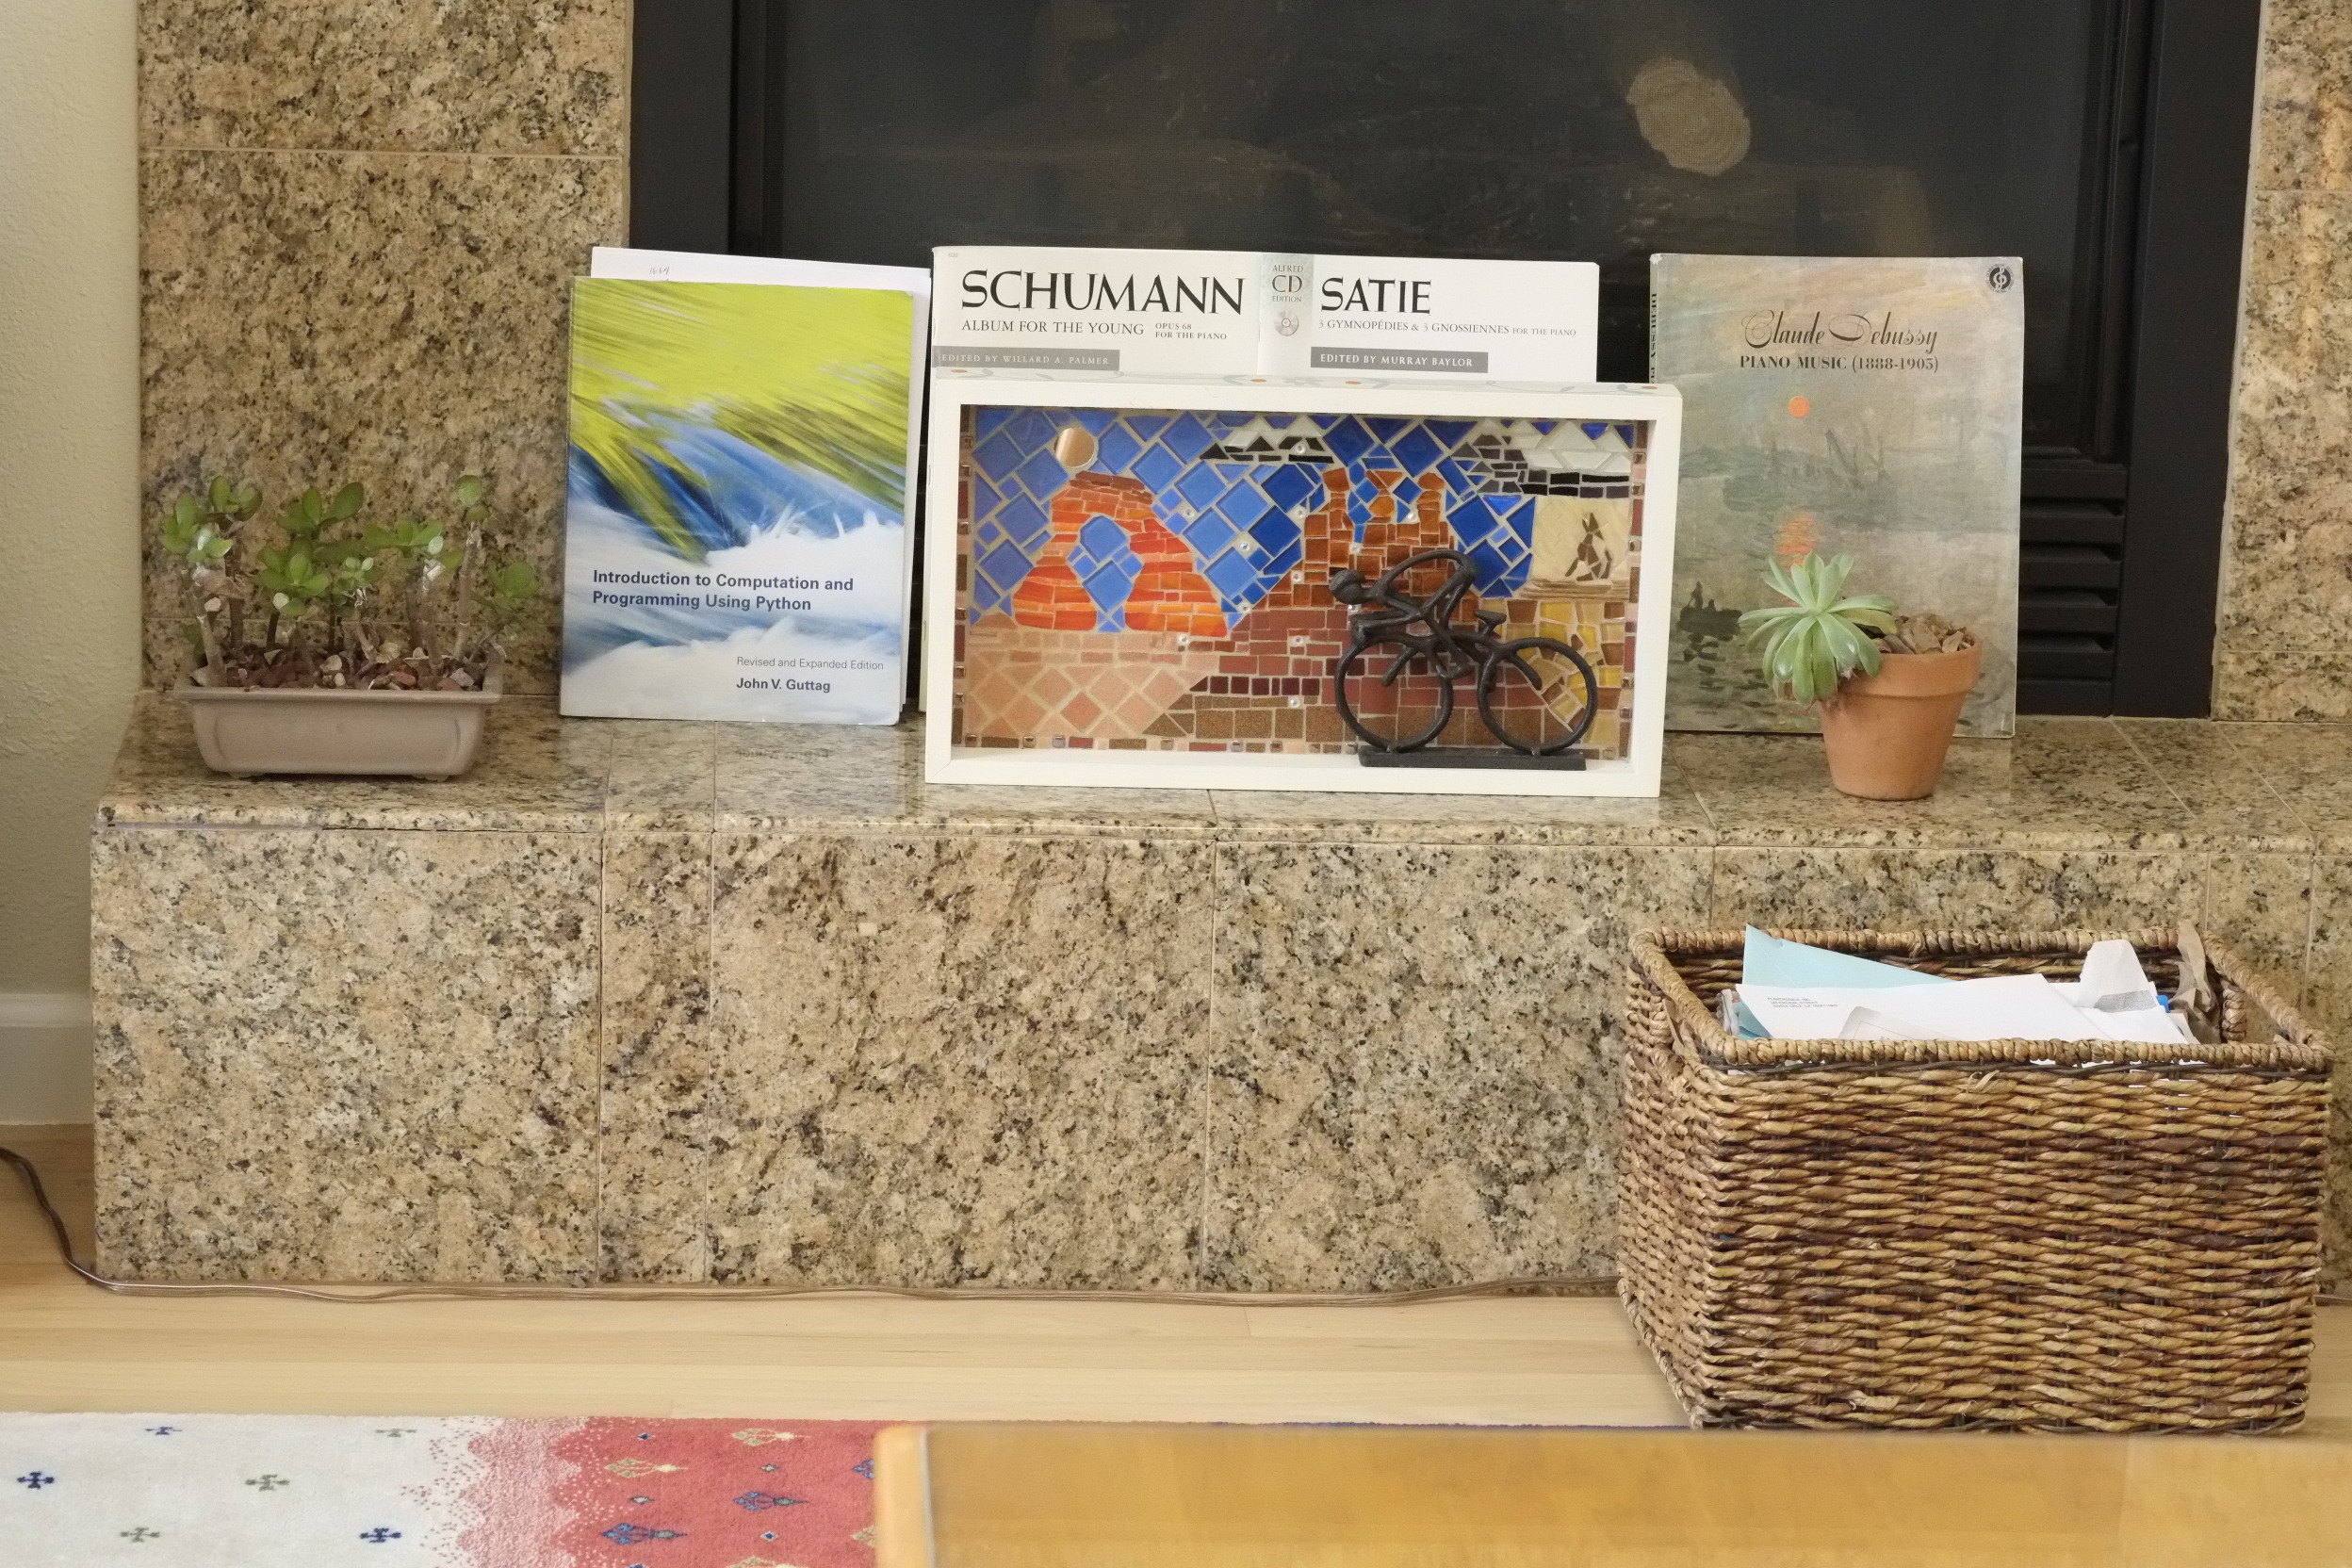
\includegraphics[width=\textwidth]{../Scene/_DSF1768.JPG}
        \caption{First scene image}
        \label{fig:sn1}
    \end{subfigure}
    \begin{subfigure}[b]{0.45\textwidth}
        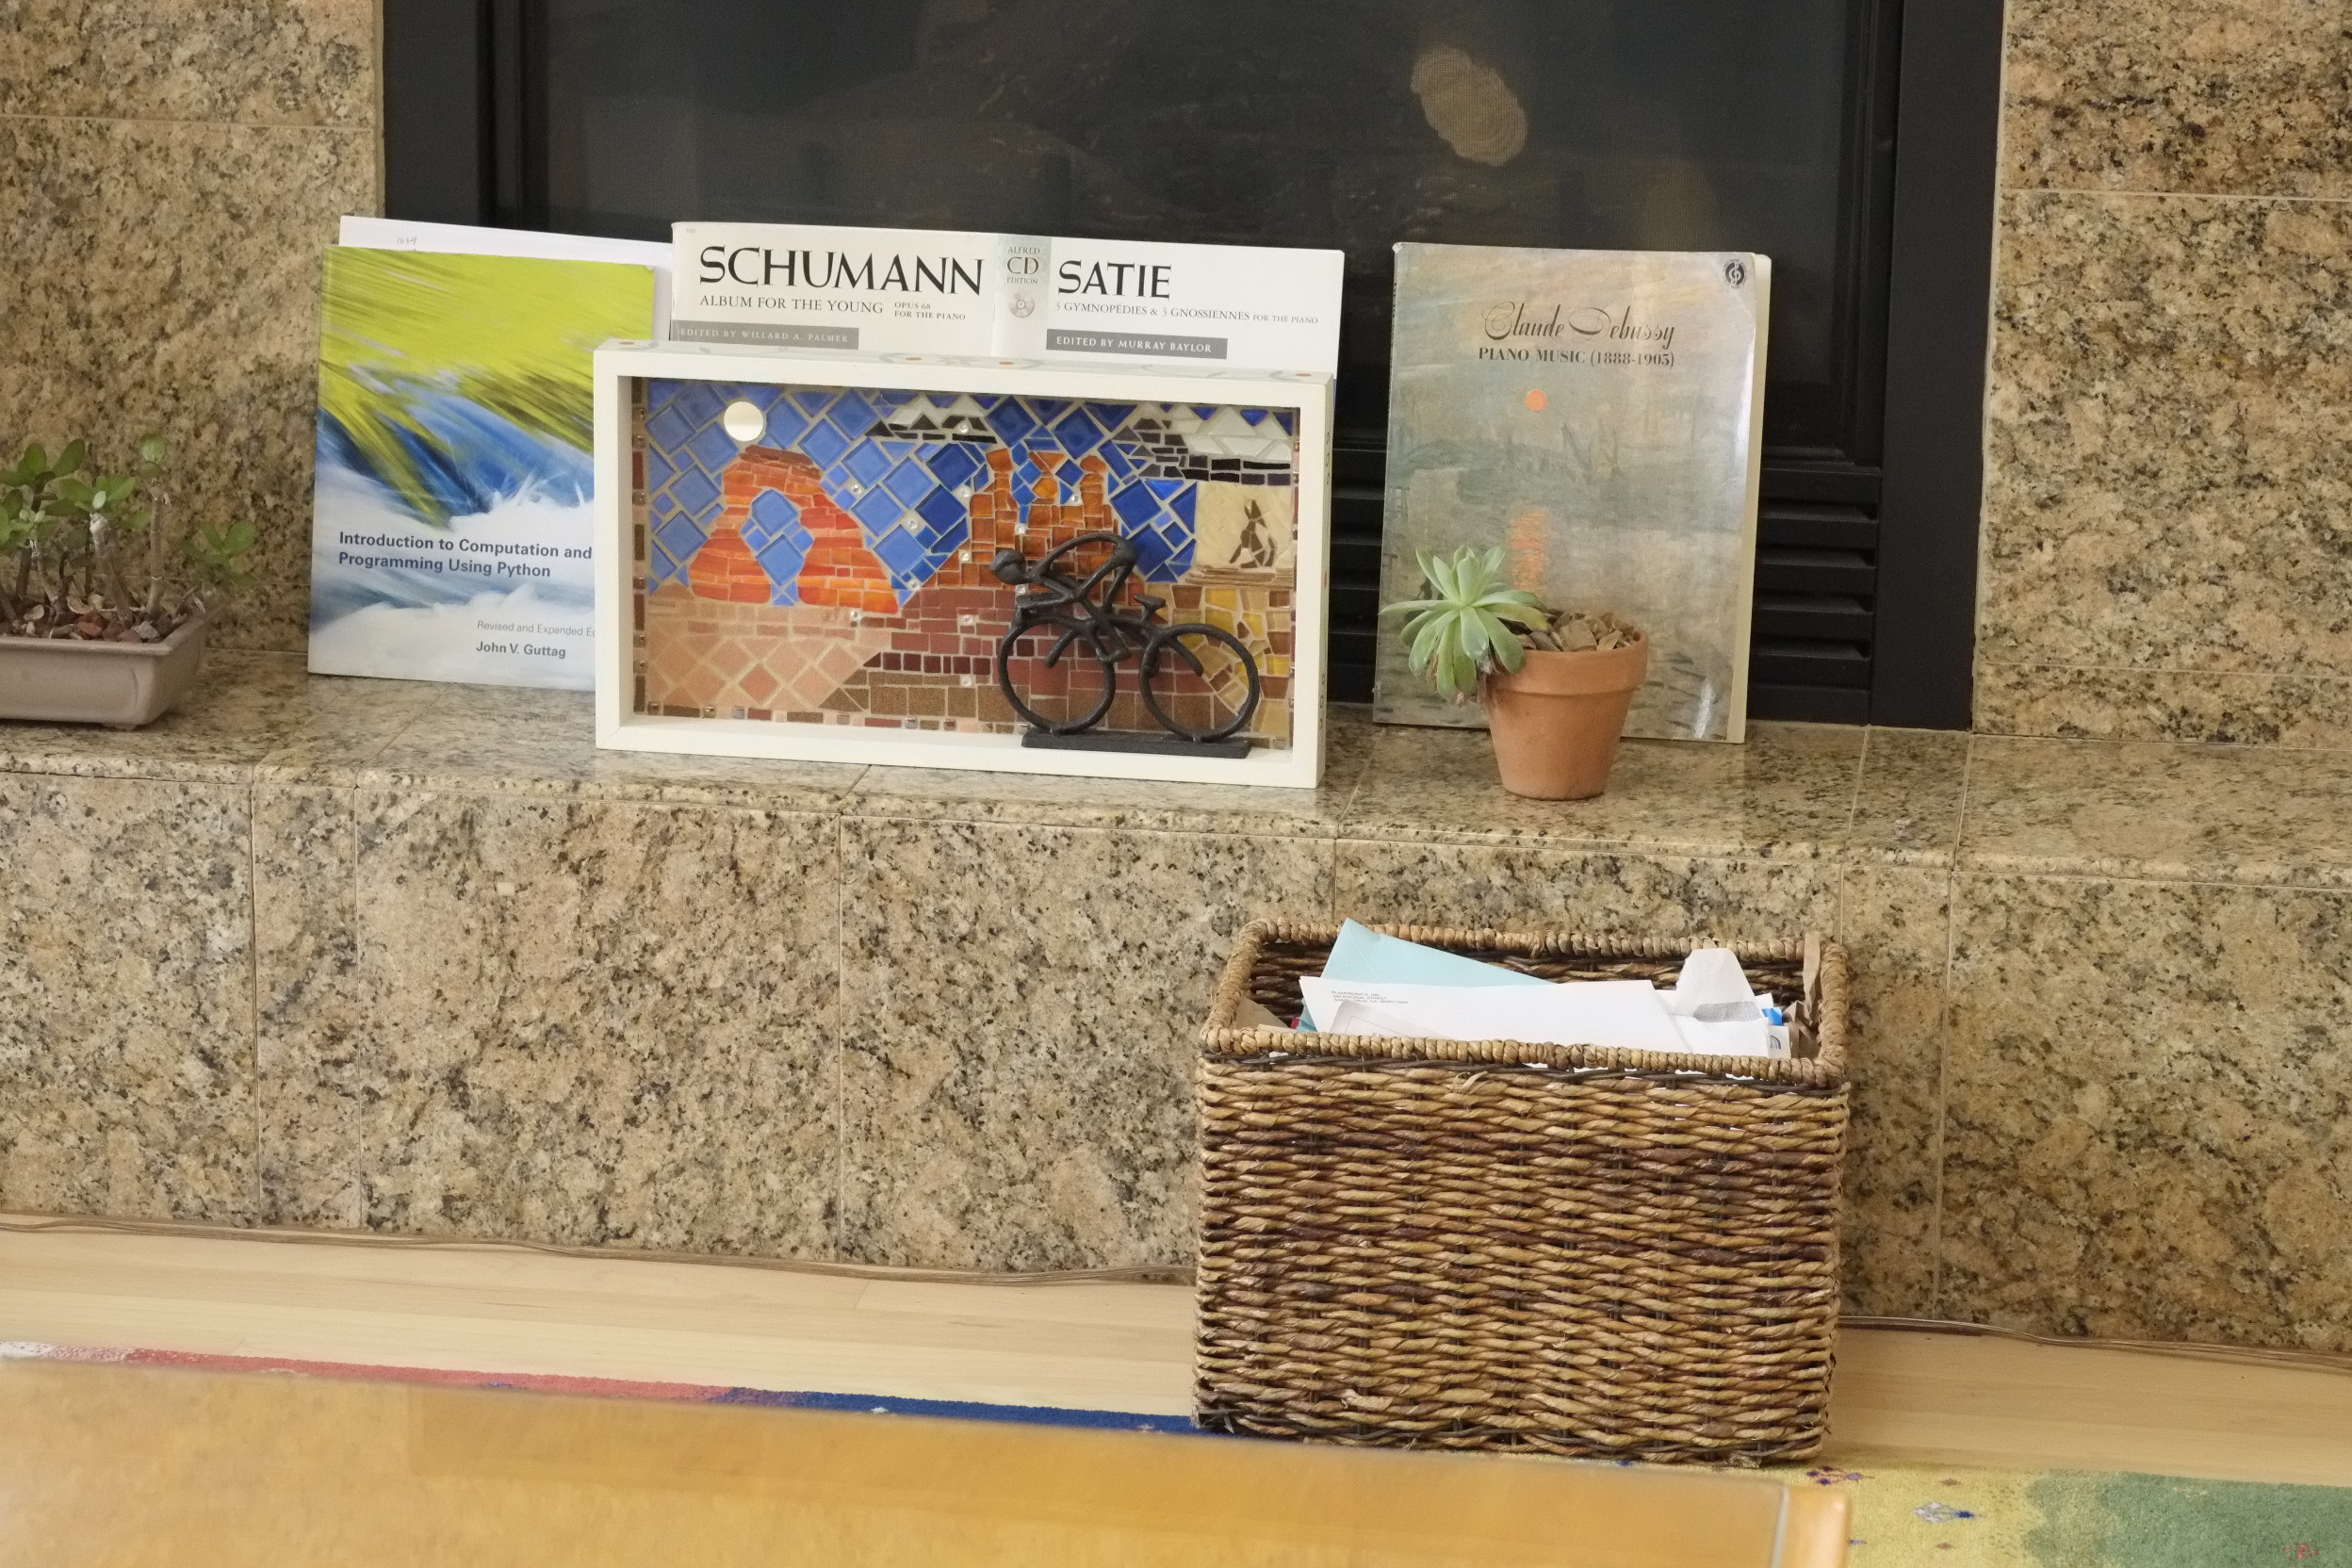
\includegraphics[width=\textwidth]{../Scene/_DSF1769.JPG}
        \caption{Second scene image}
        \label{fig:sn2}
    \end{subfigure}
\end{figure}

\FloatBarrier

%====================================Part 3=======================================
\section{Relative Camera Pose}
1.Epipolar lines
2. Write down the matrix 𝑅𝑅, 𝒓𝑅 you found. 𝐿
 3. Show the re-projected feature points on the first image
%====================================Part 4=======================================
\section{Plane Sweeping Stereo}

Deliverables:
min and max depths found
N=20 warped images
Depth image (grayscale)
%====================================Conclusions=======================================
\section{Conclusions}






\end{document}